\documentclass{article}

\usepackage{listings}
\usepackage{enumitem}
\usepackage{amsmath}
\usepackage{svg}
\usepackage{hyperref}
\hypersetup{
    colorlinks=true,
    linkcolor=blue,
    filecolor=magenta,      
    urlcolor=cyan,
    pdftitle={Overleaf Example},
    pdfpagemode=FullScreen,
    }

\title{CA Lab: Homework 4}
\author{student: Dimitri Tabatadze}

\begin{document}
    \maketitle

    \section*{Task Description} 
    
    \begin{enumerate}[label={\alph*}]
        \item {Write the code of $4\times1$ MUX in Verilog. (50 points)}
        \item {Show the timing diagram of MUX in Quartus. (40 points)}
    \end{enumerate}

    \section*{Solution}
    
    \begin{enumerate}[label={\alph*)}]
        \item {
            \begin{lstlisting}
module mux (
    input [3:0] a,
    input [3:0] b,
    input [3:0] c,
    input [3:0] d,
    input [1:0] sel,
    output reg [3:0] out);

always @ (a or b or c or d or sel)
begin
    if (sel == 0) out = a;
    else if (sel == 1) out = b;
    else if (sel == 2) out = c;
    else if (sel == 3) out = d;
end

out = (a & ~sel[0] & ~sel[0]) ^ (b & ~sel[0] & sel[0]) ^ (c & sel[0] & ~sel[0]) ^ (d & sel[0] & sel[0]);
    
endmodule
            \end{lstlisting}
        }
        \item {
            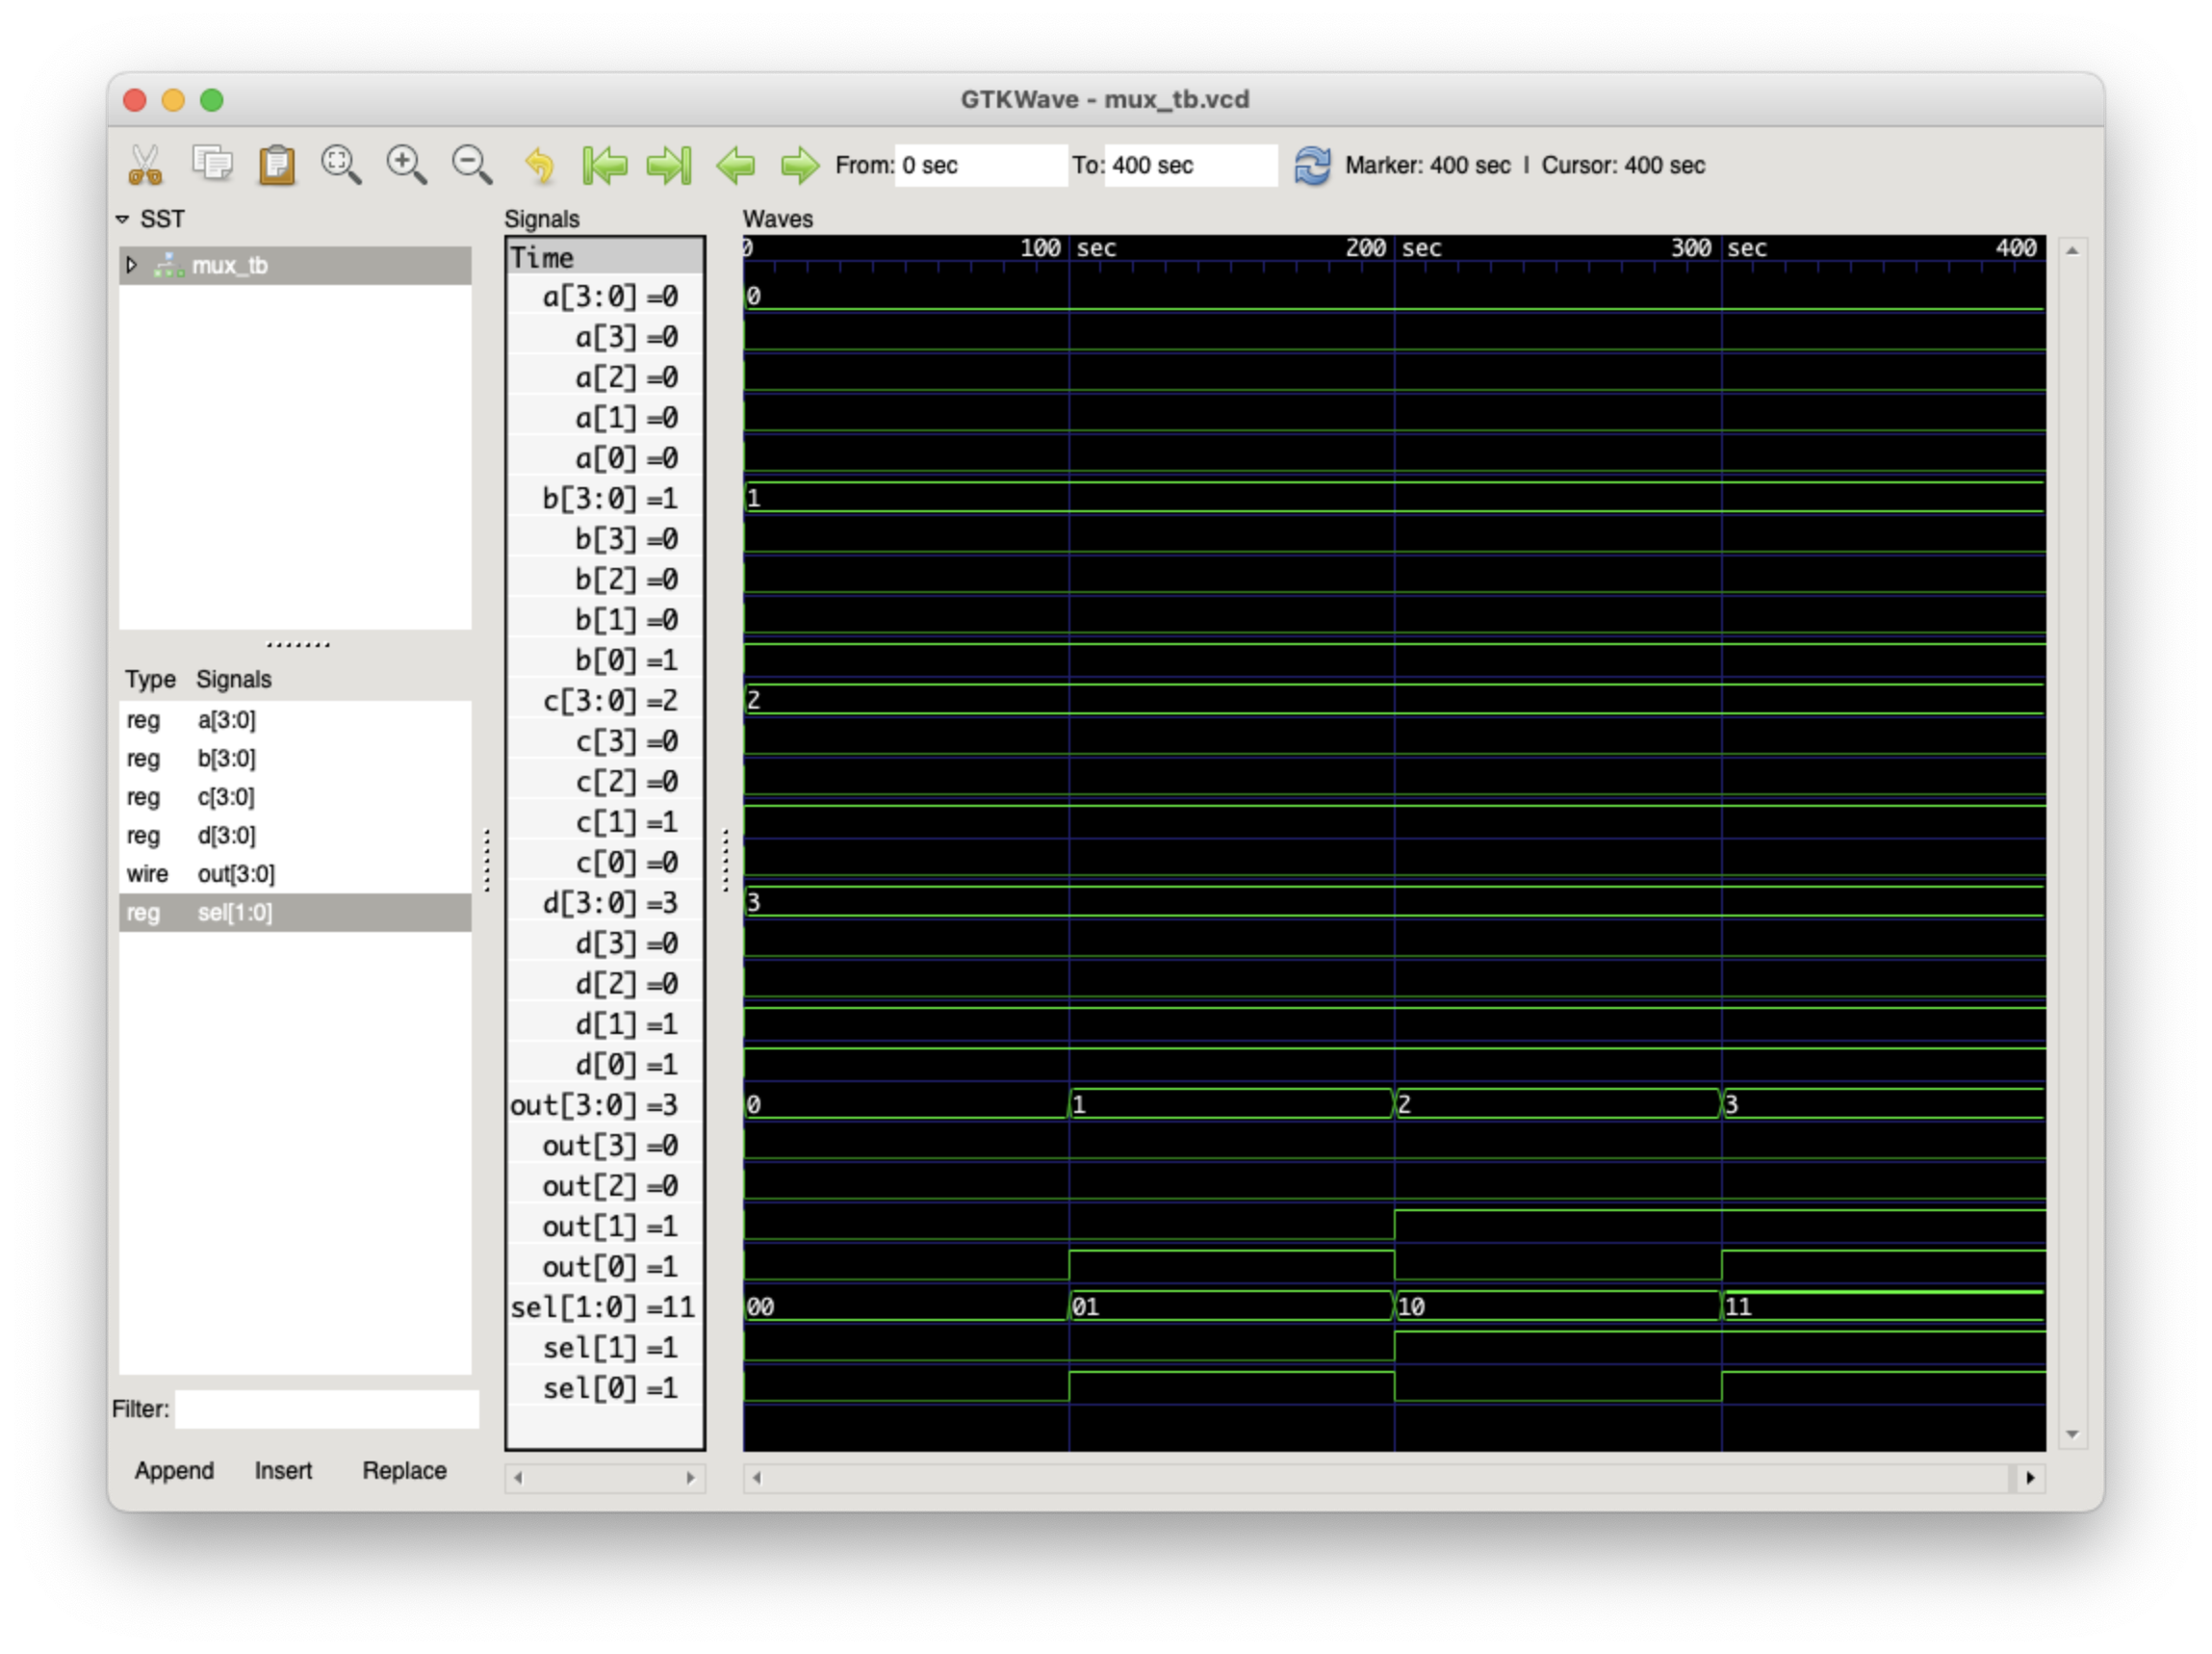
\includegraphics[width=10cm]{hw.png}
        }
    \end{enumerate}

    \section*{Conclusion}
    the homework has concluded here.
    \section*{Reference}
    there is nothing to reference.

\end{document}